\documentclass[UTF8]{ctexart}
\usepackage{mathtools,wallpaper}
\usepackage{t1enc}
\usepackage{pagecolor}
\usepackage{enumitem}
\usepackage{hyperref}
\usepackage{graphicx}
\usepackage{listings}
\usepackage{amssymb}
\usepackage[dvipsnames]{xcolor}
\usepackage{float}
\usepackage{numerica}


\begin{document}

\section{Time Complexity}
\subsection{Measuring Complexity}
\begin{itemize}
    \item 定义：M是一个确定性图灵机，确定性图灵机对所有输入都停机。确定性图灵机M的time complexity/running time是函数f：$\mathcal{N}\to  \mathcal{N} $,f(n)的意思是输入图灵机的长度为n，图灵机最多要经过多少步给出输出。如果f(n)是图灵机M的运行时间，可以说M是一个f(n)时间的图灵机。
    \item Big-O and Small-o
    \begin{enumerate}
        \item 在asymptotic analysis(渐进分析)中，我们将对算法确切运行时间的复杂表达式忽略其系数以及所有低阶项，保留时间表达式的最高阶项。
        \item 设$\mathcal{R}^{+} $是非负实数集。如果f和g是两个将$\mathcal{N} \to \mathcal{R}^{+}$的函数，如果正整数c和$n_0$存在并且每一个整数$n\geqslant n_0$使得$f(n)\leqslant cg(n)$,那么f(n)=O(g(n))。如果f(n)=O(g(n))，我们说g(n)是f(n)的asymptotic upper bound。忽略常数和低阶项后，f(n)的增长速度不会超过g(n)。
        \item Small-o notion 表示一个函数渐进意义上小于我们使用小o符号的函数。设$\mathcal{R}^{+} $是非负实数集。如果f和g是两个将$\mathcal{N} \to \mathcal{R}^{+}$的函数，如果$\frac{f(n)}{g(n)}$当n趋于无穷大的时候值为0，那么$f(n)=o(g(n))$。也就是说，对于任意实数c>0，存在一个数$n_0$,对于所有$n\geqslant n_0$的数，f(n)<cg(n)。
    \end{enumerate}
    \item Analyzing Algorithm
    \begin{enumerate}
        \item 对于图灵机$M_1$判定语言$A=\{0^k1^k|k\geqslant 1\}$的时间复杂度。
        \begin{itemize}
            \item 首先扫描整个纸带，判断是否1在0的右侧，如果1在0的左侧直接reject，扫描完后指针返回，n+n次操作，O(n)时间复杂度。
            \item 对于图灵机每次扫描，如果指针扫描第一个0时，需要寻找第一个1，每次扫描整个纸带只能删除1对01，因此扫描需要n/2次，如果每次扫描都要扫描整个纸带的元素的话，(n/2)*O(n),时间复杂度$O(n^2)$。
            \item 对于删除所有01对后，扫描整个纸带的元素进行判断，如果仍然存在0或者1，reject.O(n)
            \item 因此该图灵机是$O(n^2)$的时间复杂度。
        \end{itemize}
        \item 定义：t函数是$\mathcal{N} \to \mathcal{R} ^{+}$的映射。定义time complexity class时间复杂度类，TIME(t(n))定义为所有在$O(t(n))$时间图灵机可判定的所有语言集合。
        \item 发现：对于识别语言A的时间复杂度，依赖于计算模型的选择。
    \end{enumerate}
    \item Complexity relationships among models
    \begin{enumerate}
        \item t(n)是一个函数，并且$t(n)\geqslant n$。对于多带图灵机的每一步操作，都需要单带图灵机$O(t(n))$步进行模拟，多带图灵机每一步需要t(n)时间，那么多带到单带$O(t^2(n))$
        \item 定义：N是一个nondeterministic Turing machine并且是一个判定器(是判定器的非确定性图灵机中，对于所有输入，它的每一条计算分支都会停机，没有无线循环分支)。N的运行时间是函数f:$\mathcal{N} \to \mathcal{N}$,并且f(n)是N在输入长度为n的输入计算的任何分支上使用的最大步数。
        \item 定理：t(n)是一个函数，并且$t(n)\geqslant n$。每一个t(n)时间的非确定性单带图灵机有一个等价的$2^{O(t(n))}$ time deterministic single tape Turing machine.
    \end{enumerate}
\end{itemize}

\subsection{The class P P类}
\begin{itemize}
    \item P是在在确定性单带图灵机上能在多项式时间可判定的语言类。
    \item $P=\bigcup\limits_{k} \mathrm{TIME}(n^k)$
    \item 对于多项式等价于确定性单带图灵机的计算模型，P类是invariant不变的。
    \item P大概对应了在计算机上真实能够解决的问题类
    \item Examples of Problems in P
    \begin{enumerate}
        \item PATH问题，给定一个有向图，起点s，终点t，判断是否存在从s到t的路径？定理：$PATH \in P$, 证明PATH问题可以被确定性图灵机在多项式时间内判定
        
        定义一个图灵机M="
        在输入<G,s,t>中，G是有向图，s是起始节点，t是终点：

        (1)首先在起始节点s做标记

        (2)接着反复执行以下操作直到左右节点都被标记：每一次扫描有向图G的每一条边，如果一条边<a,b> 发现从一个标记的节点a到未标记的节点b，那么把b标记

        (3)如果t被标记，则accept，否则reject。

        "

        \item RELPRIME问题，两个数是互质如果1是能同时整除两个数的最大整数。定理：$RELPRIME \in P$
        
        使用Euclidean算法，

        E="On input <x,y>, x 和 y是自然数：

        (1)首先，执行以下算法重复y直到y=0：x=x mod y, exchange x and y

        (2)接着，输出x
        
        "

        (3)算法R解决RELPRIME， 使用E作为子程序

        R="On input <x,y>, x和y是自然数：

        (4)运行算法E，<x,y>作为输入

        (5)如果输出的值为1，accept。否则，reject。

        "


    \end{enumerate}
\end{itemize}

\subsection{The Class NP NP类}

\begin{itemize}
    \item eg1 Hamiltonian path | 哈密顿路径 | HAMPATH Problem
    
    在一个有像图G中，哈密顿路径是一条经过恰好一次经过每个节点的有向路径。

    HAMPATH={<G,s,t>|G is a directed graph with a Hamiltonian path from s to t}

    哈密顿路径问题具有多项式可验证性(polynomial verifiability)。多项式可验证性意味着验证某个问题的存在性，远比判定其存在性更加容易。验证是 核定给定解的有限性，而判定是 通过定理推导出解的pattern。

    \item eg2 合数的判定问题｜ compositeness problem
    
    若一个自然数是两个大于1的整数的乘积，那么这个数是合数。

    COMPOSITES={x|x=pq, for integers p,q >1}

    \item 定义：语言A的验证器是一个算法V，
    
    $A=\{\omega|\text{V accepts $<\omega,c>$ for some string c}\}$
    $\omega$是属于A集合的语言，c是用于验证$\omega$是属于A集合语言的辅助额外字符串。多项式时间验证器的运行时间是关于$\omega$输入长度的多项式运行时间。若语言A存在多项式时间验证器，那么称A是多项式可验证的。c是certificate证书。

    \item 定义:NP(Nondeterministic polynomial time)是具有多项式时间验证器的语言类。P类是NP类的子集。
    \item NTM求解HAMPATH
    
    $N_1=$"<G,s,t>作为输入，G是有s节点和t节点的有向图，
    \begin{enumerate}
        \item 生成一个m个数字的列表，m是有向图的节点个数。每一个在列表中的数都是不确定性被选择(为了同时覆盖所有可能)在1到m之间。
        \item 检查列表是否含有重复项，如果发现重复项，则拒绝。(淘汰重复的无效分支)
        \item 检查是否$s=p_1$且$t=p_m$，如果失败，则拒绝。(保证起点和终点符合要求)
        \item 对于每一个i在1到m-1之间，检查是否$(p_i,p_{i+1})$是有向图G的边，如果不是则拒绝，如果全部通过则accept。
    \end{enumerate}

    "

    \item 定理:一个语言属于NP类当且仅当这个语言能够被某个非确定性多项式时间图灵机所确定。
    
    推导。我们设：A可由多项式时间非确定性图灵机N判定，V是根据NP类定义所存在的用于语言A多项式时间验证器，V是运行时间为$n^k$的图灵机。

    N="在输入长度为n的w上
    \begin{enumerate}
        \item 非确定选择字符串c，并且c的长度不超过$n^k$。批量生产所有可能的certificate。$n^k$确保验证过程能在多项式时间内完成。
        \item 运行V在输入<w,c>
        \item 如果一个V分支 accept，accept；否则如果所有V的分支都拒绝，则拒绝。
    \end{enumerate}
    "

    V="在输入<w,c>,w和c均为字符串（有点像For+if+break）
    \begin{enumerate}
        \item 在输入串w上模拟非确定性图灵机N的运行（验证器V是确定性图灵机，要还原N度非确定性计算过程）。证书c的每一个字符都对应着N在计算遇到的每一个非确定性选择点。
        \item 如果N的计算过程分支接受，则V接受，否则拒绝。
    \end{enumerate}
    "

    \item 定义：NTIME(t(n))={L|L is a language decided by a O(t(n)) time nondeterministic Turing machine}。NP=$\cup_k$NTIME($n^k$)
    \item clique问题。在无向图中一个clique是一个子图，其中在任意两个节点都有一条边相连。一个k-clique是一个包含k个节点的clique。Clique问题是去确定是否一个图包含指定大小的团。
    
    CLIQUE=\{<G,k>|G is an undirected graph with a k-clique\}
    
    CLIQUE属于NP问题。clique是证书。

    证明：

    V="在输入为<<G,k>,c>:
    \begin{enumerate}
        \item 检验c是否是G中k个节点组成的集合
        \item 验证是否G包含所有连接c中节点的所有边
        \item 如果全部通过，则accept；否则拒绝
    \end{enumerate}
    "
    N="在输入为<G,k>:
    \begin{enumerate}
        \item 非确定性地选择G中的k个节点的子集clique
        \item 验证是否G包含连接这个clique的所有边
        \item 如果有一个通过，则接受；如果全部不通过，reject。
    \end{enumerate}
    "
    
    \item P vs NP Problem
    
    \begin{enumerate}
        \item P类问题是可以在多项式时间内判定某字符串是否属于该语言的语言构成的集合
        \item NP类问题是可以在多项式时间内验证某字符串是否属于该语言的语言构成的集合
    \end{enumerate}

\end{itemize}

\subsection{NP-Completeness NP完全性}
\begin{itemize}
    \item Cook-Levin理论：如果某一类特定的 NP 问题存在多项式时间算法（P=NP），那么所有 NP 问题都能找到多项式时间算法。SAT是NP-complete，3SAT是NP-complete
    \item SAT问题，可满足问题，satisfiability problem。一个可满足问题是去检验是否一个布尔公式是可满足的。如果对布尔公式的变量进行0和1的赋值使这个公式值为1我们称这个布尔公式可满足。
    
    SAT=\{<$\phi$>|$\phi$ is a satisfiable Boolean formula\}

    \begin{enumerate}
        \item 定理：SAT$\in$P iff P=NP
    \end{enumerate}
    
    \item Polynomial Time Reducibility多项式时间可归约性
    \begin{enumerate}
        \item 定义：一个方程f:$\sum^* \to \sum^*$(从由字符集构成的字符串集合映射到字符集构成的字符串集合)是一个多项式时间可计算函数，如果某个多项式时间图灵机M存在并且对于任何输入w,图灵机M都会在停机时在读写纸带上写下f(w)。简单来说：函数f是多项式时间可计算函数，如果存在一台多项式时间图灵机M满足，给M输入f的任意一个输入字符串，M会在多项式时间内停机，并且停机时，它的读写带上只有f(w)这一个字符串输出。
        \item 定义：若存在一个多项式时间可计算函数f:$\sum^* \to \sum^*$，使得对每一个w存在$w \in A \Longleftrightarrow f(w)\in B$,则称语言A多项式时间映射可归约到语言B，记作$A \leqslant_P B$.
        \item 定理：如果语言A多项式时间可归约到B，并且B属于P类，那么A属于P类。if $A \leqslant_P B$ and $B \in P$, then $A \in P$.
        
        假设M是判定B的多项式时间算法，f是从A到B的多项式时间归约，我们描述一个多项式时间算法N判定A：

        N：“对于输入w
        \begin{enumerate}
            \item 计算f(w)
            \item 使用f(w)作为输入，运行M，输出M输出的内容。
        \end{enumerate}
        ”

        \item A literal 字面量
        
        \begin{enumerate}
            \item 字面量是布尔表达式的变量及其取反的布尔变量。
            \item clause（子句）是布尔变量使用析取符号（并集）进行连接的表达式子。如果若干子句通过合取符号（交集）进行连接的表达式子，我们称之为合取范式(conjunctive normal form/cnf).
            \item 如果有3个子句构成的合取范式，则称为3 cnf-formula。
            \item 定理：首先我们定义一个3SAT=\{<$\phi $>|$\phi $ is a satisfiable 3 cnf-formula \}在可满足的3合取范式中，每一个clause都包含至少一个被赋值为1的字面量。\textbf{3SAT is polynomial time reducible to CLIQUE}。
            
            证明的关键是构造一个多项式时间转换函数f，把3SAT的输入(公式$\phi $)转换成CLIQUE的输入且满足：$\phi $是satisfiable 能够推出图G中存在大小为k的团，$\phi $是unsatisfiable 能够推出图G中不存在大小为k的团
            \begin{enumerate}
                \item 假设$\phi $是一个带有k个子句的函数：$\phi =(a_1\lor b_1\lor c_1)\land (a_2\lor b_2\lor c_2)\land ... \land (a_k\lor b_k\lor c_k)$。把k个子句拆成3个节点的k组三元组，并从k组节点中挑选k个节点，要满足：同一个三元组内节点不相连(SAT要求每个子句满足赋值后结果为1，因此在转换时我们要从k个子句中每一个子句仅挑选一个节点)，矛盾字面量不相连(如果一个组中$x_k$=1，那么$x_k$取反在另一个子句中出现要是0，这样$x_k$就矛盾了。)
            \end{enumerate}
        \end{enumerate}
        
    \end{enumerate}

    \item NP完全性的定义
    \begin{enumerate}
        \item 定义：一个语言是NP-complete 如果满足两个条件
        \begin{enumerate}
            \item B是在NP类中
            \item 在NP类中的A是多项式时间归约到B
        \end{enumerate}
        \item 定理：如果B是NP-complete并且B属于P，那么P=NP。
        
        证明：根据B的定义，每一个在NP类中的A是多项式时间归约到B，B又属于P类，那么A同样属于P类，根据Cook-Levin定理，推出P=NP。

        \item 定理：如果B是NP-complete 并且$B\leqslant_{P} C$对于NP类中的C，那么C是NP-complete。
        
        证明：我们已知B是NP完全，那么NP类中的A都可以在多项式时间归约到B，由于语言B又可以在多项式时间内归约到C，因此A可以在多项式时间内归约到C，C是NP-complete。

    \end{enumerate}

\end{itemize}

\subsection{Additional NP-Complete Problem}

\begin{itemize}
    \item 在构造从3SAT问题到某一语言的多项式时间归约时，我们需要寻找该语言中能够模拟布尔公式里变量和子句的结构，这种结构叫做gadget(构件)。
    \item Vertex Cover Problem顶点覆盖问题
    
    若G为无向图，G的顶点覆盖是满足如下条件的顶点子集：图G的每条边都至少与该子集中的一个顶点相关联。简单来说，就是图G的所有边占有的不同的图G中的节点。$VERTEX-COVER=\{<G,k>|G is an undirected graph that has a k-node vertex cover\}$。

    \begin{figure}[H]
        \centering
        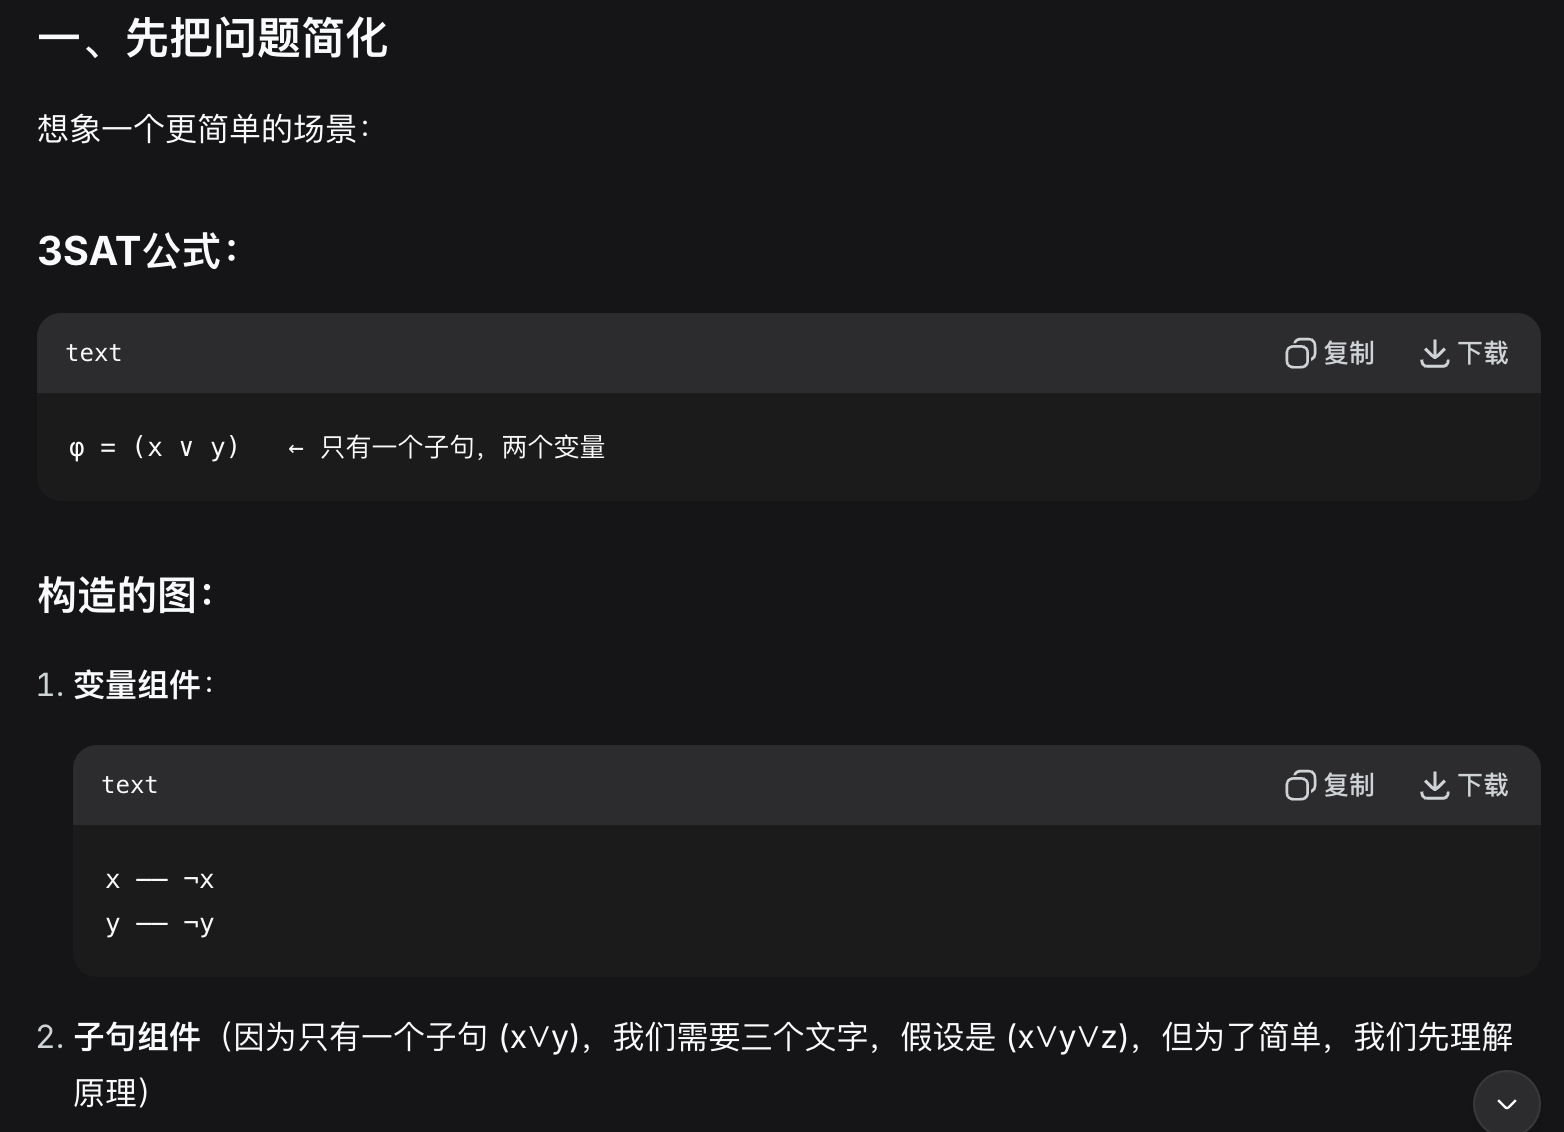
\includegraphics[width=0.55\textwidth]{static/Vertex-Covereg1-1.png}
        \caption{Vertex-Covereg1-1}
        \label{Vertex-Covereg1-1}
    \end{figure}

    \begin{figure}[H]
        \centering
        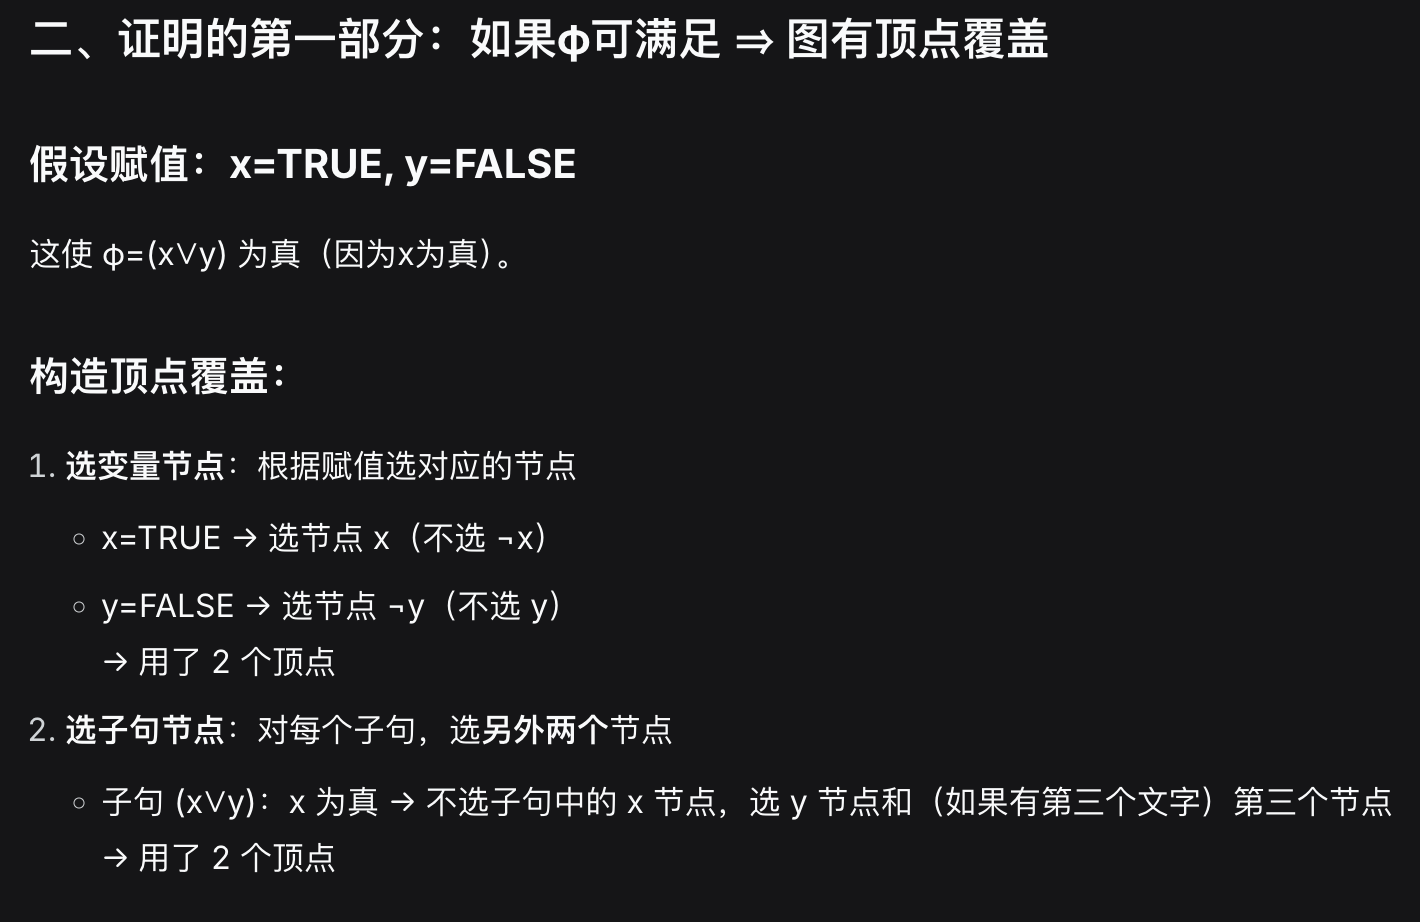
\includegraphics[width=0.55\textwidth]{static/Vertex-Covereg1-2.png}
        \caption{Vertex-Covereg1-2}
        \label{Vertex-Covereg1-2}
    \end{figure}

    \begin{figure}[H]
        \centering
        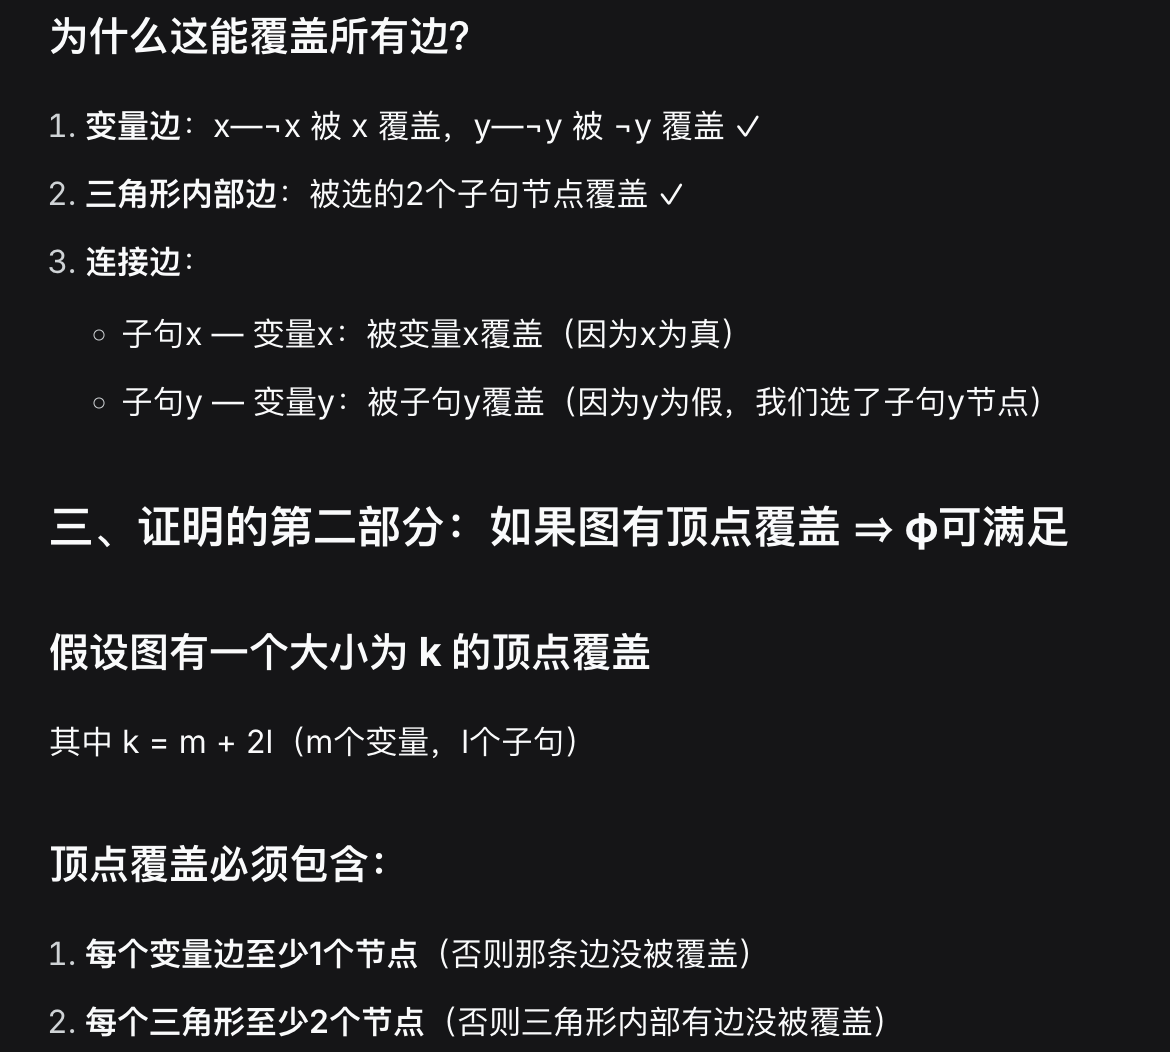
\includegraphics[width=0.5\textwidth]{static/Vertex-Covereg1-3.png}
        \caption{Vertex-Covereg1-3}
        \label{Vertex-Covereg1-3}
    \end{figure}

    \begin{figure}[H]
        \centering
        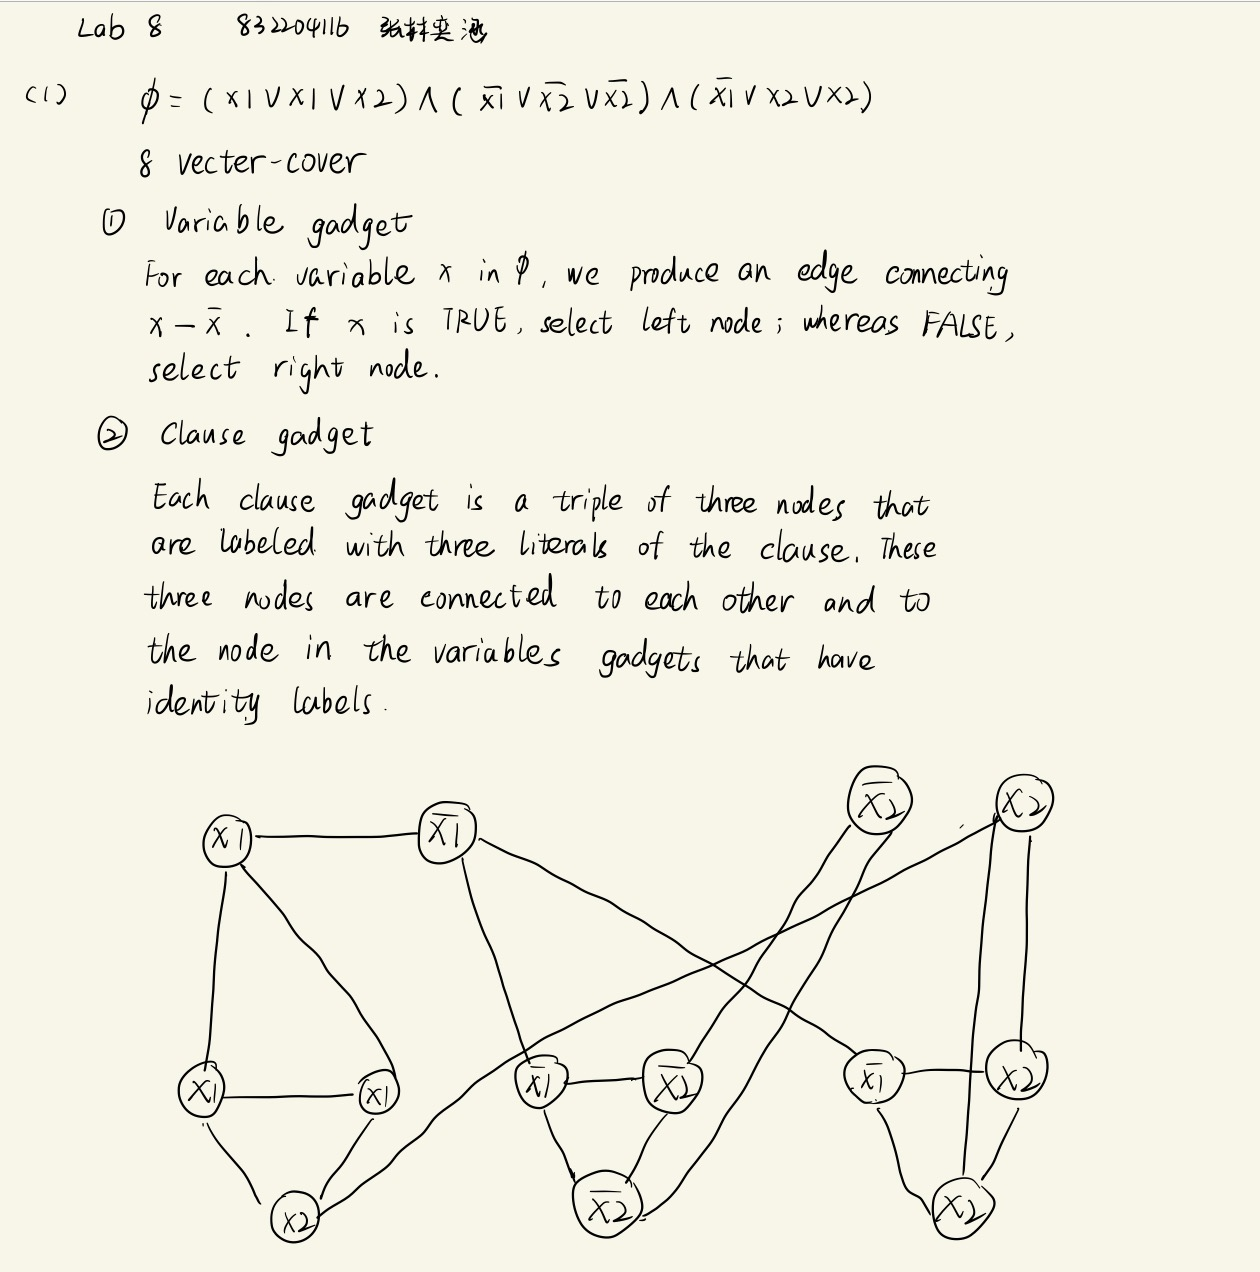
\includegraphics[width=0.5\textwidth]{static/Vertex-Covereg2-1.jpg}
        \caption{Vertex-Covereg2-1}
        \label{Vertex-Covereg2-1}
    \end{figure}

    \begin{figure}[H]
        \centering
        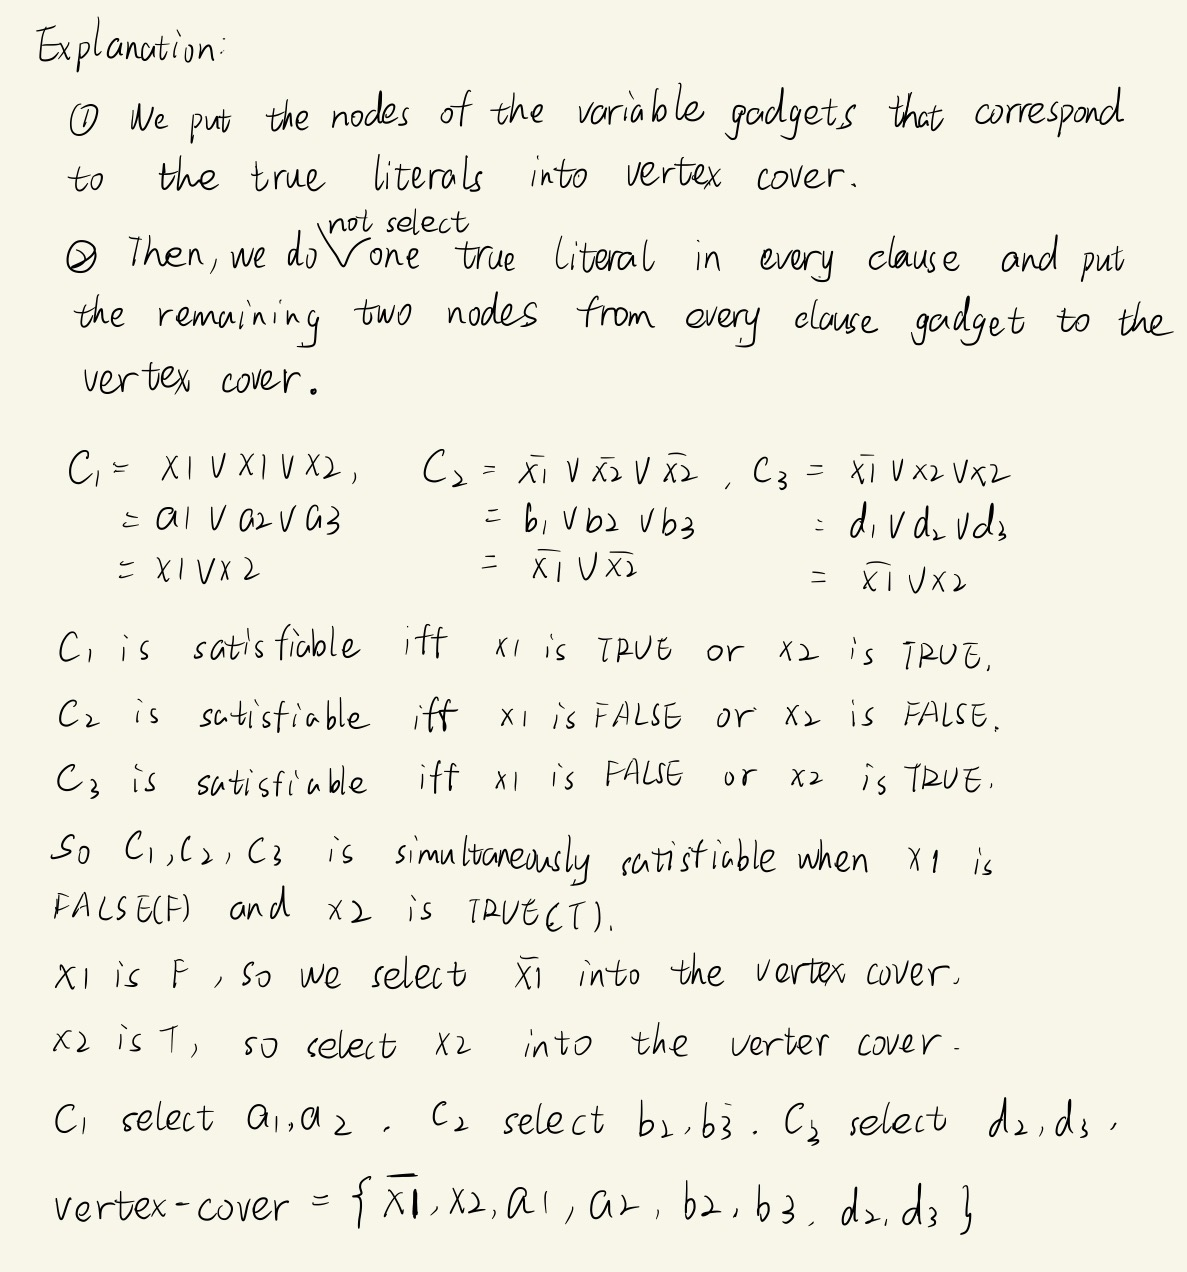
\includegraphics[width=0.5\textwidth]{static/Vertex-Covereg2-2.jpg}
        \caption{Vertex-Covereg2-2}
        \label{Vertex-Covereg2-2}
    \end{figure}

    \begin{figure}[H]
        \centering
        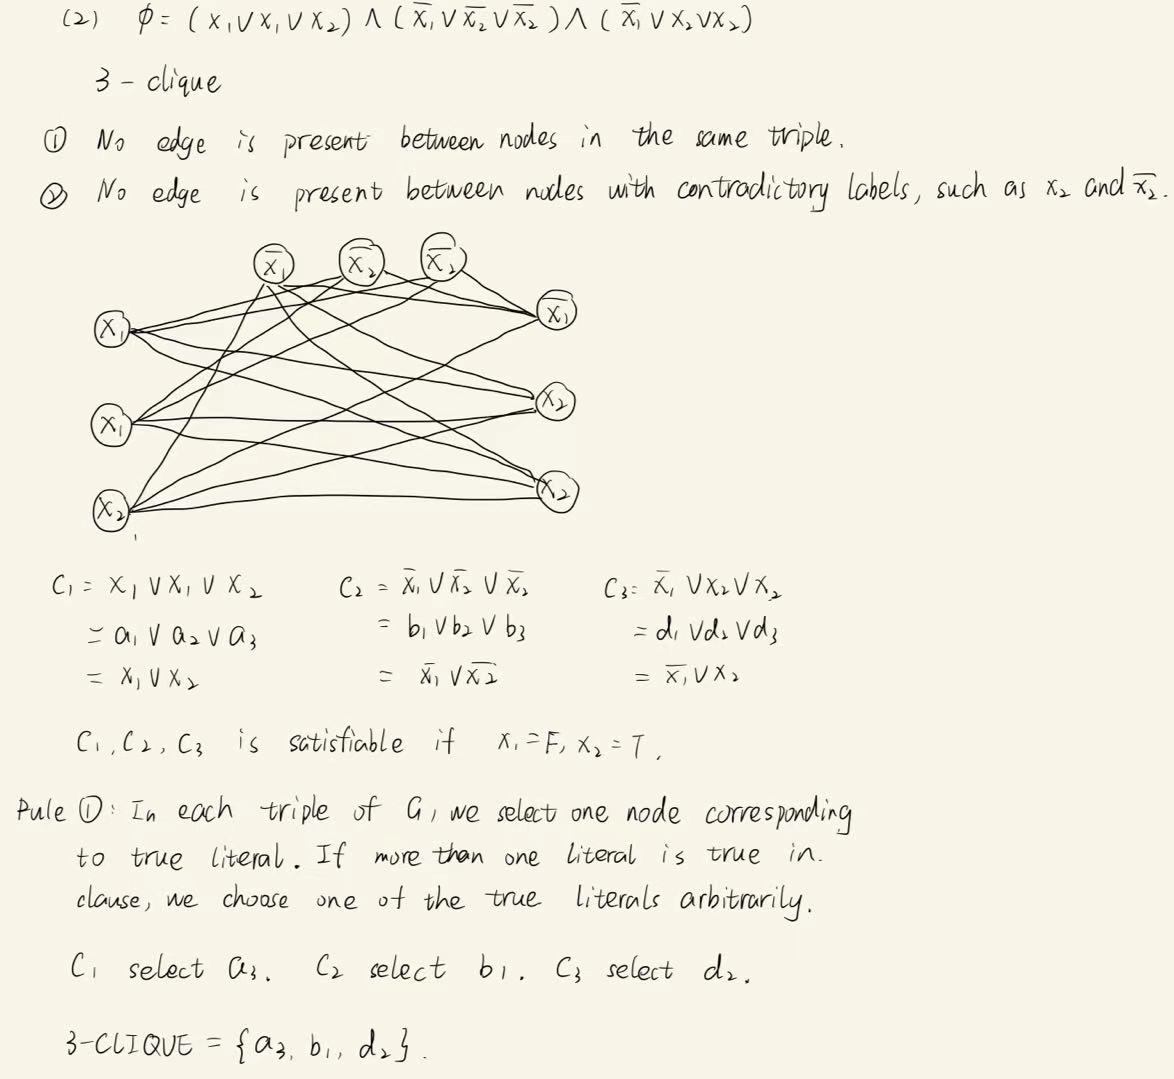
\includegraphics[width=0.5\textwidth]{static/Vertex-Covereg3.jpg}
        \caption{Vertex-Covereg3}
        \label{Vertex-Covereg3}
    \end{figure}

\end{itemize}


\end{document}